\documentclass{sig-alternate-10pt}
\usepackage{graphicx}
\usepackage{balance}
\usepackage{comment}
\usepackage{times,epsfig,subfigure,endnotes,color,url,paralist,multirow,float}
\usepackage{epstopdf}
\usepackage[pdftex]{hyperref}
\hypersetup{
	pdftitle={SIGCHI Conference Proceedings Format},
	pdfauthor={LaTeX},
	pdfkeywords={SIGCHI, proceedings, archival format},
	bookmarksnumbered,
	pdfstartview={FitH},
	colorlinks,
	citecolor=black,
	filecolor=black,
	linkcolor=black,
	urlcolor=black,
	breaklinks=true,
}

\begin{document}

\title{A Comparative Study of MobilityFirst and NDN towards ICN-Centric Internet of Things Architecture}

\numberofauthors{1}
\author{
\alignauthor
Sugang Li\winlab, Yanyong Zhang\winlab, Dipankar Raychadhuri\winlab
\vspace{2mm}
Ravi Ravindran\huawei, Guoqiang Wang\huawei
        \vspace{2mm}
        \affaddr{{\winlab}WINLAB, Rutgers University, North Brunswick, NJ, USA}
          \vspace{1mm}
        \affaddr{{\huawei}Huawei Technologies, Santa Clara, CA,USA}       
}

\maketitle

\begin{abstract}

Internet of Things (IoT) promises to connect billions of objects to Internet. After deploying many stand-alone IoT systems in different domains, the current trend is to develop a unified IoT platform so that objects can be made accessible to applications across organizations and domains. Towards this goal, quite a few proposals have been made to build a unified IoT platform as an overlay on today�s Internet. Such an overlay solution, however, is inadequate to address the important challenges posed by a unified IoT system, especially in terms of mobility, scalability, and communication reliability, due to the inherent inefficiencies of the current Internet. To address this problem, we propose to build a unified IoT platform based on the Information Centric Network (ICN) architecture, which we call ICN-IoT. ICN-IoT leverages the salient features of ICN, and thus provides seamless mobility support, scalability, and efficient content and service delivery. Specifically, we explore using two ICN architectures -- MobilityFirst and NDN --  to support IoT, and refer to them as MF-IoT and NDN-IoT, respectively.   

In this paper, we discuss the detailed design of MF-IoT and NDN-IoT, focusing on their service discovery and pub/sub model. For evaluation purpose, we consider two realistic IoT applications scenarios, a smart building scenario and a smart campus bus scenario, with the former representing mostly stationary IoT devices while the latter representing mobile IoT devices. We have also compared the performance of these two approaches through detailed simulations. 

\end{abstract}

\section{Introduction}
\label{sec:intro}

During the past decade, many stand-alone Internet of Things (IoT) systems have been deployed, in domains including smart homes, smart grids, smart transportation, smart healthcare, etc.  The recent trend is to evolve towards a globally unified IoT platform, in which billions of objects connect to the Internet, available for interactions among themselves, as well as interactions with many different applications across boundaries of administration and domains.  Building a unified IoT platform, however, poses a set of unique challenges on the underlying network and systems. To name a few, it needs to support a large number of networked objects\cite{***},  many of which are mobile. These objects will have  heterogeneous means of connecting to the Internet, often with severe resource constraints. Further, interactions between the applications and objects are often real-time and dynamic, requiring strong security and privacy protections.  To address these challenges, we next identify several key requirements of a unified IoT system. 

Cisco predicts there will be around 50 Billion IoT devices such as sensors, RFID tags, and actuators, on the Internet by 2020~cite{***}. The first step towards a unified IoT platform,  is thus the ability to assign names that are unique,  secure, and persistent against  dynamic attributes that are common in IoT systems, such as device mobility.   Further, the underlying platform needs to scale smoothly with respect to the number of devices and the amount of data generated by these devices.  Another challenge for IoT systems is the resource constraints faced by many IoT devices, including constrained resources in power, computing, storage, bandwidth, etc.  Specifically, power constraints limit how much data the devices can process and communicate,  computing constraints limit the type and amount of processing the devices can perform, storage constraints of the devices limit the amount of data that can be stored on the devices, and  bandwidth constraints limit the amount of communication these devices can have. Finally, a unified IoT platform should be able to provide seamless services  in the presence of device mobility.  

%\input{requirement}
% ICN IoT Architecture Requirement 
%\input{naming}
%Naming Assignment and name resolution
\section{Device/Service Discovery}\label{sec:discovery}
Device discovery is one outstanding benefit when we deploy IoT system on ICN network.In the traditional IP-based IoT system, in order to use human-readable or application-readable name to identify sensing and actuating device, middleware usually handle name to IP/PORT address mapping, with the IP transport oblivous of application delivery. And the middleware can be complex and require amount of development time. IoT entities have been typically identified using manufacturer assigned IDs, which can be cryptographic ID, human readable name etc.These names are mapped to its locator-ID and used as de-facto IDs in the Internet today, that has issues with dynamic properties such as mobility. In contrast, ICN can use these natives IDs without any further mapping, and scale control and forwarding overhead through active participation by the network. Middleware somehow will be less significant as it is in IP network.  
%Look for jeff's paper here

In NDN lighting system\cite{},it assumes that lighting device comes with a manufacture assigned public key, a shared secret for initialized authorization, and a well-known NDN name, such as /ndn/lighting for discovery. First, a new device register itself and publish its public key.The configuration manager(CM) will periodically express its interest using a well-known service name, such as ndn/lighting. If a node connect to a new device, it reply a corresponding data packet with new device information. Lastly, the CM assigns a application-specific name, authenticates fixture by a shared secret.    

\subsection{Device/Service Discovery in Mobilityfirst}\label{sec:discoverymf}
In MobilityFirst IoT architecture, we embrace locator/ID split technique for device mobility.Also, device/service separation design is introduced here to support current low power device in a homogeneous network environment.We assumes that all IoT devices only carry a manufacturer serial number, which could be used to derive a GUID from Name Certificate and Resolution Service(NCRS)\cite{}.The IoT end device access point(EDAP), i.e. sink,fixture or even mobile phone for wearable sensor, utilize GUID to identify their service type, such as environment sensing,light control or health sensing.Once a new device attaches to a sink or fixture, it will announce its serial number as GUID, EDAP performs a GNRS insert with entry of Device GUID -> Service GUID mapping. A configuration service(CS) running on the remote server query GNRS server with Service GUID periodically. If the new device has been inserted by EDAP, query result will contain certain GUIDs.
\begin{figure}
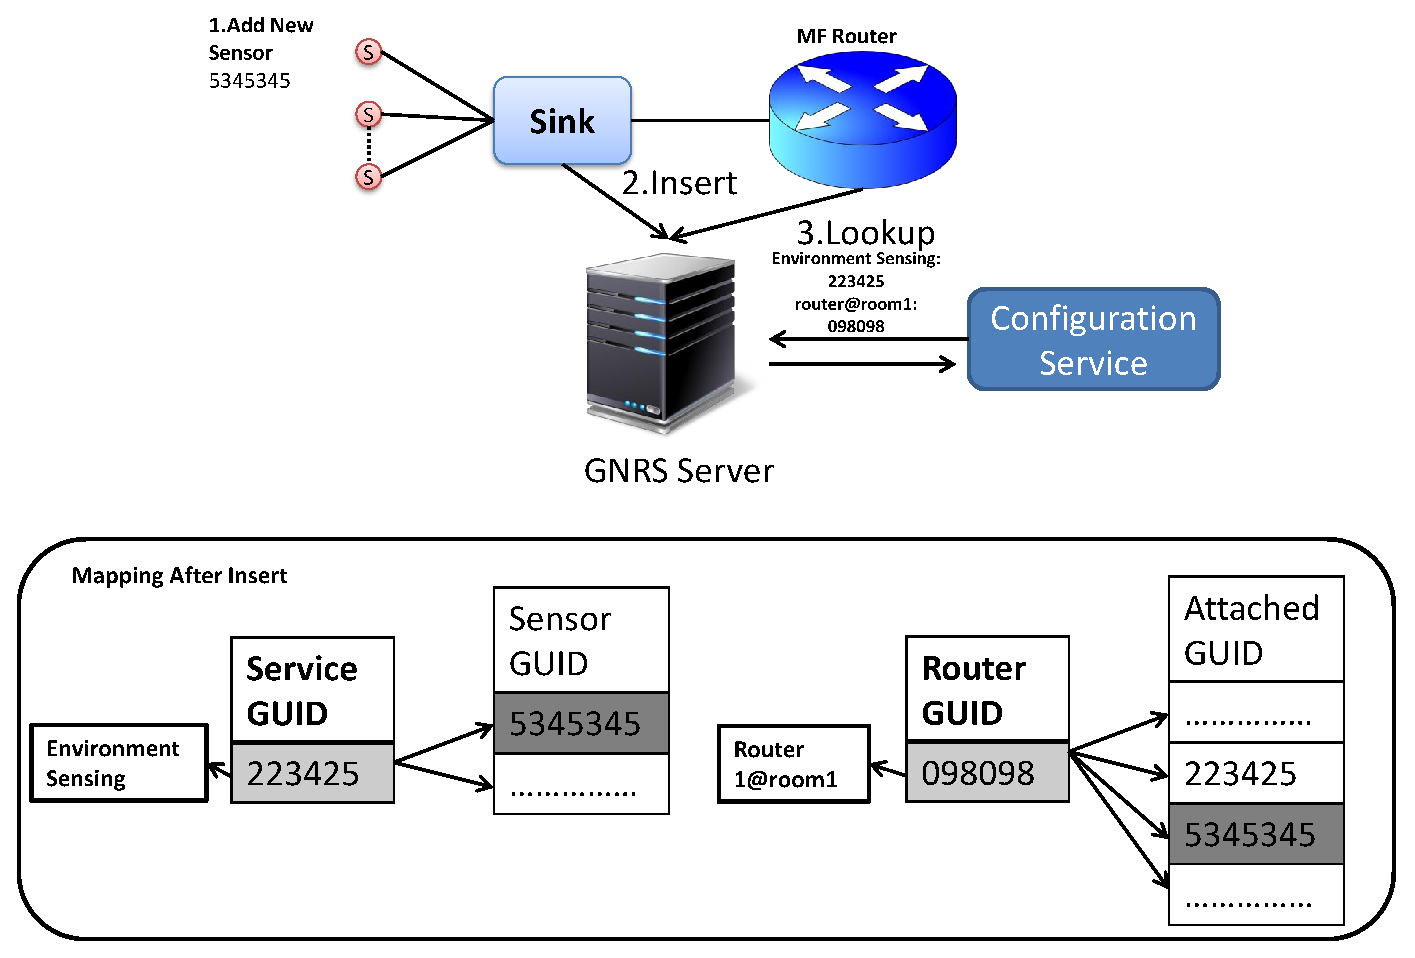
\includegraphics[width=3.00in,height=2.00in]{discovery.eps}
\caption{Three Steps for Discovery}
\label{fig:disc}
\end{figure}
Shown as Figure ~\ref{fig:disc}, a new wireless sensor dispose in a room, express itself with serial number 12345 to the nearest EDAP. EDAP is powered and relative consistent, so that we can pre-configure the service type for the it, i.e. assign a GUID or use its serial number to represent the service type. Once EDAP receive the message from the new sensor, it first looks up the local stack to confirm it has not been added before. Sensor GUID(12345) -> Service GUID(67890) mapping is inserted to GNRS server, if it does not exist in local stack. Configuration Service periodically looks up for  Service GUID(67890), and the new GUID(12345) will be  in the result list if it has been inserted. In our example, since the low power sensor has limited bandwidth and store cache, its GUID can be consistent and require no dual-way authentication. After checking the local database, CS register the new device to the IoT server if it has not being stored, in which resource and subscription membership being managed.
%do we need to include the authentication process for other device?

          

%For example, a new temperature wireless sensor comes with a serial number 1234, attaches to a EDAP, i.e. a sink node. The GUID of the sink node represents a certain service type  temperature sensing
\section{Data Dissemination in ICN}\label{pubsub}
Publish/Subscribe model is a comment approach in IoT system for resource sharing and management. In traditional IP network, most of the IoT platforms provide a centralized server to aggregate all IoT device resources, publish them to the web portal,and manage the subscribing membership. The subscriber may need to retrieve the sensor data from the server. Such centralized architecture no doubt can benefit the accessibility for each device. However, scalability and bandwidth consumption due to control and data information exchange may be a significant issue, if billions of IoT devices involve. Thus, a decentralized publish/subscribe model might be needed to solve this challenge.

Content-Oriented Pub/Sub System (COPSS)\cite{} achieve an efficient pub/sub capability for CCN. It integrates a push based multicast module with the pull based CCN architecture at the content-centric layer.

\subsection{Pub/sub in MobilityFirst}
To maintain the convenience of traditional centralized Pub/Sub model and reduce the bandwidth consumption, we propose the Pub/Sub model in MF IoT platform.In order satisfy requirement of different applications, we provide two communication model--push and pull mode for sensor data retrieval in MobilityFirst.

\subsubsection{Basic Push Mode}
In many IoT applications, data transmission is event-driven, where sensor or sink tends to update itself to the server as specific event is detected.For instant, smoke sensor will be triggered only when smoke is detected, it needs to update the monitoring application in the shortest time. In this case, a push-based low latency data transmission approach is necessary.    As what we introduce above, Configuration Service registers the all devices in the IoT server, where subscription membership is managed. Taking security and MobilityFirst multicast into account, we introduce a new type of GUID -- Subscription GUID(sGUID) here. Besides identifying devices, application and content in the MF network, GUID can also be used to establish a subscription relationship. 

When a application subscribes to a web service that providing sensor resources over the IoT server, a sGUID will be assigned to it and listened as a destination GUID. Single Subscription GUID can be assigned to multiple applications, if they subscribe to the same sensor resource. The sink of the subscribed sensor will be notified with the Subscription GUID.Without knowing the GUID of application,sink set this sGUID into the destination GUID field in a MF header, and begin to send sensor data. Taking advantage of GSTAR\cite{} routing protocol and host protocol stack\cite{} in MF, whenever a receiver announce a new GUID being listened, its MF access router performs a GNRS insert and add it to local routing table. Therefore, if different clients announce they listen at the same sGUID, the nearest MF router performs a multicast so that all of them can receive data from source sensor. For example, shown as Figure~\ref{fig:pubsub}, application $GUID=789$ subscribes to sensor $GUID=123$ on IoT server. $sGUID=456$ will be assigned to both the sink and application. At the sink side, sGUID will be set as destination GUID, whenever sensor updates to the sink, this data will be sent to $sGUID=456$. The MF access router will be updated if host announces a new GUID is added to the listening list. Since GUID is consistent in the network, such approach utilize locator/identifier split mechanism of MF, where locator here is the GUID of the MF access router. Mobility of both the client and application running on it can be handled properly.   
%update the figure to show the sensor,table, and routing table. 
\begin{figure}
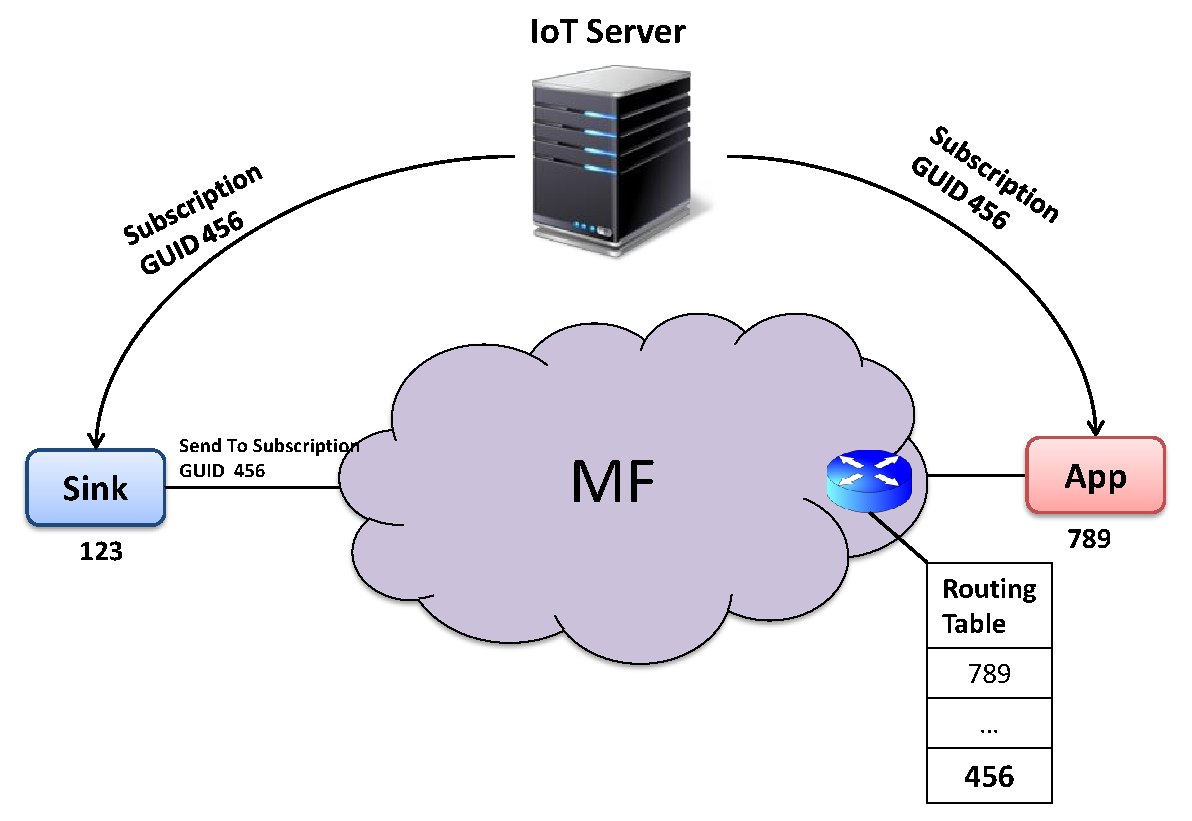
\includegraphics[width=3.00in,height=2.00in]{pubsub_push.eps}
\caption{Basic Push Mode on MF IoT}
\label{fig:pubsub}
\end{figure}

\subsubsection{On Demand Pull Mode}
In ICN architecture, where we include the concept of data consumer and producer, data transmission is on-demand--it is driven by the interest from data consumer, and data producer respond per request. Instead of a single sensor, application sometimes tends to subscribe to a certain service, which may include a group of sensors.Therefore, a sensor data retrieval method in MF is proposed to enable application pulling sensor data based on certain criteria or context.

Besides basic one-to-one data request and reply communication, we would like to introduce a mechanism where multiple sensor objects can be access via one sink node, so that many-to-one or one-to-many capability can be achieved. To associate a group of sensor with a subscriber application, we can make use of the Subscription GUID, in order to reduce the complexity of the information for the subscriber application. In order words, it can send data request to multiple sensors on multiple sinks by single Subscription GUID. However, the question is when the sink receive the message via the a single sGUID, how can it learn which sensors that application want exactly? IoT server needs to provide more hints to the sink node. Shown as Figure~\ref{}, we establish a relationship between the sensors and the application in the IoT server. Similar to the basic push mode we discuss above, IoT server assigns a message with sGUID followed by multiple sensor GUIDs which is in the subscription, so that sink node can understand the exact sensor objects to access. Since every request packet contains the GUID of the applicaton, sink nodes can respond to it without querying any third party service. 
%We assume that IoT server already knows  the service GUID and locator GUID(GUID of the router), which already contain certain context information from name assignment service.
% For example, since sink node is relatively stationary and aggregates limited types of sensor,the service GUID can represent the environment sensing, as well as the identifier for the sink. IoT server use the service GUID and router GUID to look up in the GNRS server. In respond, two lists of GUID will be sent back to IoT server. After comparing these two lists,IoT server can obtain the desired group of sensor GUIDs. Furthermore, 

%make a figure for IoT server finding sensor guid andt sink application pulling data from sink node.
\begin{figure}
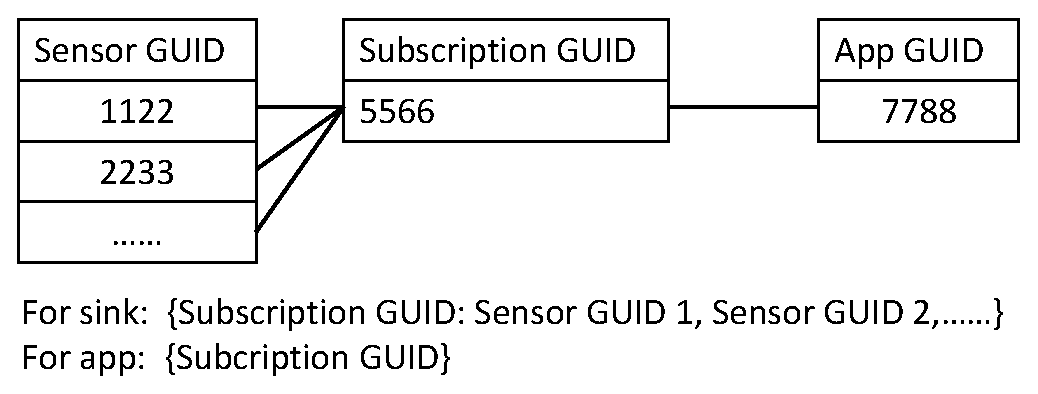
\includegraphics [width=3.00in,height=1.30in]{two_step_pull.eps}
\caption{Mapping Relationship}
\end{figure}
\section{Application Scenarios}
IoT area covers a wide range of applications, and each of them can be varied from each other on system requirement.To better evaluate the capability of underlying ICN network, we need to design and deploy both classical and challenged IoT application scenario over ICN network. Therefore, we choose smart campus as a starting point, because it has a reasonable scale and most of the design can be easily fit into a larger scale scenario, such as smart city.
\subsection{Buidling Management System}
In the past decade, to solve the huge energy consumption issue and provide a intelligent building facility monitor and control service, building management system (BMS) has been developed and standardized  by both academia and industry. In a smart campus scenario, especially a campus as big as Rutger  University, BMS plays a significant role in taking control of a complex ecosystem such as climate control, security monitoring,smoke detection and so on. Most of these system running on heterogeneous communication protocol, and we will like to inter-connect them with homogeneous network protocol and enable the reachability by using name or identifier. 
\subsubsection{Architecture Design}
Given that BMS provides a User Interface for control operation and monitoring, but most of the traffic is generated by device self reporting, which means it is a data-producer-driven system.For example, thermostat adjustment is triggered by the fluctuated data reading from a temperature sensor and motion sensor will inform light switch when movement is detected. 

We classify the net devices into four types-- sensing device, core network device, BMS server, and actuating device. The sensing device here is the sink which has full network stack  and aggregates the data from wireless sensor network (WSN). In order to provide reachability of low power sensor and flexibility of sensor data retrieval, the sink maintains each sensor as an object or content. These objects can either be updated to BMS server by the sink directly, or be pulled by remote data consumer on demand. The actuating device is basically full-network-stack thermostat or light fixture, which provide a network interface for air conditioner or light bulb. The system architecture is shown as Figure~\ref{fig:bms_arch}. Environment monitoring service,occupation monitoring service and control service are running on BMS server to enable building automation. 

To simplify our system design, we refer to Building Automation and Control Network (BACnet) protocol~\cite{}, which has been standardized by  American Society of Heating, Refrigerating and Air Conditioning Engineers (ASHRAE), and applied in many commercial BMSs. Based on BACnet, we define the objects we mention above as the format shown in Table~\ref{}.Although BACnet is application layer protocol that requires middlleware to provide a mapping from name to specific network address(NA), we substitute the identifier with ICN name. The only difference between MF and NDN is the name field, where we use GUID and NDN name respectively. 
%change the icon of humity sensor, bulb, and AC. 
\begin{table}
\label{tab:bac_object}
\end{table}
\begin{figure}
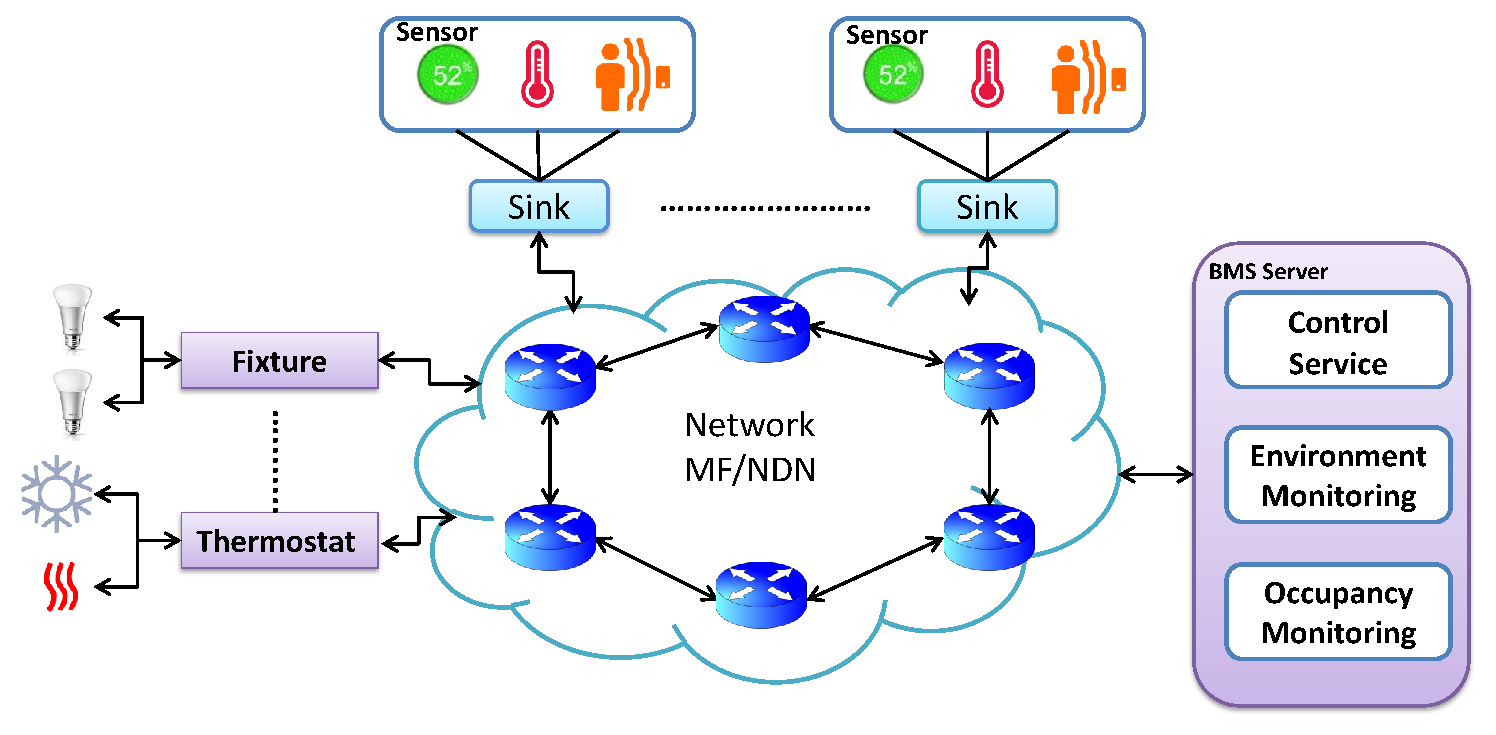
\includegraphics[width=3.1in,height=2.00in]{bms_arch.eps}
\caption{BMS over MF/NDN}
\label{fig:bms_arch}
\end{figure}
\subsubsection{One BMS Example of Device Discovery}
Since thousands of IoT devices are installed in buildings on campus, daily maintenance and configuration could be very complicated and time-consumed. With device discovery mechanism in MF, this task can be completed with less manual operation.

Assumed a new temperature sensor needs to be added to the big conference room in WINLAB, Rutgers University. It comes with a manufacturer serial number, which can also be used as its GUID (sensorGUID). The sink installed in this room is named with serviceGUID, representing service type "Environment Sensing". It connects to the nearest MF access router identified with rGUID, which stands for "Router@conferenceroom". As we discuss above, sensorGUID->serviceGUID mapping and sensorGUID->rGUID mapping will be inserted into GNRS server when the sink begins to receive message from the sensor. Configuration Service which periodically send look up for serviceGUID, and find the new device after comparing the result list with the local exiting devices list. As long as CS discover this new device, it exposes to the BMS server for further operation.
 
\subsection{School Bus System}
Another interesting scenario in a campus scenario is school bus system. It operates over the whole campus day and night, which thousands of students and faculties benefits from it. Now the increasing integration of sensors into vehicles makes a intelligent interactive school shuttle information system become possible.Specific applications such as fleet management system and NextBus system have been developed to provide a more efficient and convenient transportation service for the public. 

A smart bus system should provide network interfaces from vehicle  to infrastructure (V2I), and infrastructure to user.  Currently, the most common network device on bus is Mobile Data Terminal (MDT), which is a GSM-based communication module supporting data exchange between control center and bus via SMS. Most of vehicle support Controller Area Network bus (CANbus) protocol\cite{}. It enables sensors on vehicle can communicate with each other without a host computer. Also, sensor data such as velocity, seat occupation,and GPS obtained by CANbus can be transmit to the infrastructure via MDT directly. However, there are certain limitation on this type of communication model. First, SMS has constraint format of data, multimedia information from on-bus camera or microphone need to be transmitted in alternative way. Second, there is a significant delay from several seconds to several minutes via SMS per transmission, that make a real-time vehicle update become unrealistic. Since school bus operates in a wifi-covered campus, we assume that all shuttle routes are closed enough to the wifi access points. In a IP wifi network, given that the delay issue has been solved, mobility become a new challenge.Therefore, we propose a ICN infrastructure based school bus system (SBS) to evaluate the performance of both MF and NDN in dynamic environment.
\subsubsection{Architecture Design}
In our ICN based school bus system,  shown as Figure~\ref{},we dispose either MF Mobile Data Terminal(mMDT) or NDN (nMDT) Mobile Data Terminal on each bus respectively. To simplify our evaluation, we only choose three types of sensor which are relatively popular to user and system administrator -- velocity sensor, seat sensor, and GPS. Along with the bus route, enough number of access points are installed to provide seamless wifi coverage.Similar to our BMS design, a centralized SBS server handles updates from MDT, as well as sends notification to all buses or single bus. In order to support some specific application, we also need to evaluate the peer-to-peer communication in a V2I architecture. 
\begin{figure}
\includegraphics[width=3.1in,height=2.00in]{school_bus.eps}
\caption{Route A \& School Bus System Architecture}
\label{fig:bus}
\end{figure}
\subsubsection{Pub/Sub in The Same Route}
To give a example that combine both mobility and pub/sub in MF, we introduce a information sharing mechanism in the school bus system.  Supposed that drivers in Rutgers Bus Route A(shown in Figure~\ref{fig:bus}) interest in the position and occupancy of other buses among the same route. They subscribe to the "Route A Data Sharing from Bus\#1" service, and obtain a subscription GUID (subGUID) from server to listen.The access routers they attach will add this subGUID to the routing table and insert subGUID -> routerGUID mapping to the GNRS server.As the sender, Bus\#1 send position and occupancy information to the subGUID. If the packet arrives at the edge router, but the bus has moves to the next access point, the packet will be stored locally based on GSTAR protocol. The router then performs a GNRS lookup for for the latest NA (GUID of the access router) of the subGUID, and forward the packet to this NA.      
 
\subsection{Smart Parking System}
\section{Evaluation}
\subsection{Stationary IoT Scenario}
\begin{figure}
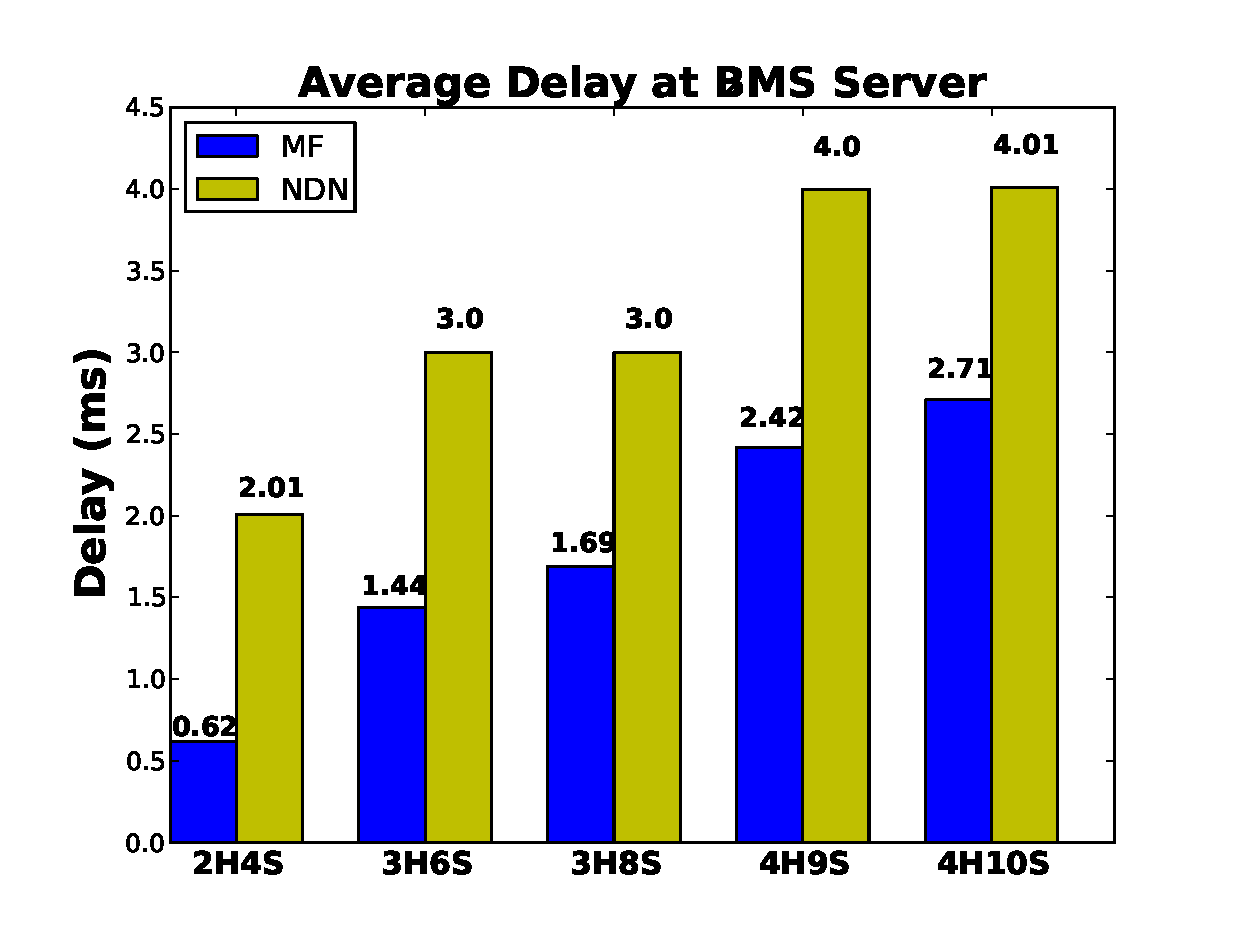
\includegraphics[width=3.00in,height=2.00in]{ave_delay_server.eps}
\caption{Average Delay on BMS server}
\end{figure}
\begin{figure}
\includegraphics[width=3.00in,height=2.00in]{throughput_ndn_mf.eps}
\caption{Throughput at BMS Server}
\end{figure}

\subsection{Dynamic IoT Scenario}

%\input{relatedwork}
%\input{conclusion}

\balance
\scriptsize
%\footnotesize
%\small

%\bibliography{../bibtex/sugang}
\end{document}